\documentclass[12pt, a4paper]{article}
\usepackage[utf8]{inputenc}
\usepackage[spanish]{babel}
\usepackage{csquotes}
\usepackage[style=apa,backend=biber]{biblatex}
\addbibresource{./referencie.bib}
\usepackage[T1]{fontenc}
\usepackage{amsmath}
\usepackage{amsfonts}
\usepackage{booktabs}
\usepackage{float}
\usepackage{amssymb}
\usepackage[a4paper, margin=2.54cm]{geometry}
\usepackage{setspace}
\usepackage{titlesec}
\usepackage{graphicx}
\usepackage{pgfplots}
\usepackage{pgf-pie}
\usepackage{booktabs}
\usepackage{enumitem}
\usepackage{pdflscape} % Para landscape
\usepackage{multirow} % Para combinar celdas
\usepackage{array} % Para ajustar anchos de columnas
\usepackage{listings}
\usepackage{xcolor}
\usepackage{pdfpages}
% Configuración de listings
\lstset{
    language=Python,           % Lenguaje de programación
    basicstyle=\ttfamily\small, % Estilo básico
    numbers=left,              % Numeración de líneas
    numberstyle=\tiny\color{gray},  % Estilo de los números
    stepnumber=1,              % Paso para la numeración
    frame=single,              % Marco alrededor del código
    breaklines=true,           % Dividir líneas largas
    captionpos=b,              % Posición de la leyenda
    showstringspaces=false,    % No mostrar espacios en cadenas
    backgroundcolor=\color{lightgray!10}, % Color de fondo
    keywordstyle=\color{blue}, % Estilo de palabras clave
    commentstyle=\color{green!60!black}, % Estilo de comentarios
    stringstyle=\color{red}    % Estilo de cadenas
}
\renewcommand{\arraystretch}{1.5} % Ajusta el espaciado entre filas
% Configuración de APA 7ma edición

\setlength{\parindent}{0.5in}
\titleformat*{\section}{\normalfont\bfseries}
\titleformat*{\subsection}{\normalfont\bfseries}
\titleformat*{\subsubsection}{\normalfont\bfseries}
\pgfplotsset{compat=1.18}


\begin{document}
\onehalfspacing

\begin{titlepage}
    \begin{center}
        \vspace{0.5in}
        \small “Año del Bicentenario, de la consolidación de nuestra Independencia, y de la conmemoración de las heroicas batallas de Junín y Ayacucho”
  
        
        \Large Universidad Nacional Hermilio Valdizán
        
        \Large Facultad de Economía
        
        \vspace{0.5cm}
        
        \begin{figure}[h!]
            \begin{center}
                
\includegraphics[width=0.40\textwidth]{images/unheval.jpg}
                \hspace{0.5cm}  
                
\includegraphics[width=0.45\textwidth]{images/economia.png}
            \end{center}
        \end{figure}
        
        \Large{Brecha digital en estudiantes universitarios: Análisis descriptivo en la Facultad de Economía - Unheval 2024}
        \vspace{0.5cm} 

        \large\textbf{Docente:}

        \large\textbf\author{Cueva Laguna, Jeel E. }
        

        \large\textbf{Autores:}

        \large\textbf\author{Chavez Huaranga, Jorge}

        \large\textbf\author{Chuquiyauri Tordecillo, Ronaldhino M.}

        \large\textbf\author{Nieto Serpa, Luis}

        \large\textbf\author{Palomino Ricaldi, Antony R.}        
        
        \large\textbf\author{Rojas Benancio, Delsy}

        \large\textbf\author{Valentín Baquerizo, Dan Jhu Ali}
        
        \large\textbf\author{Villanueva Herrera, Tony}
        
        \vspace{0.5cm}
        
        \Large Huánuco - Perú 
        
        \large 2024
    \end{center}
\end{titlepage}


\tableofcontents
\newpage

\begin{abstract}
La investigación analiza la brecha digital en los estudiantes de la Facultad de Economía de la Unheval durante el ciclo académico 2024-2, enfocándose en las desigualdades de acceso, uso y habilidades relacionadas con las TIC. Estas limitaciones afectan el rendimiento académico y la preparación profesional en un entorno cada vez más digitalizado.

El objetivo principal fue analizar la brecha digital considerando las dimensiones de acceso, uso y habilidades digitales, evaluando factores como conectividad, frecuencia de uso y competencias en herramientas tecnológicas.  

La metodología adoptó un enfoque cuantitativo y descriptivo. Se aplicó un cuestionario a una muestra representativa de 72 estudiantes seleccionados de una población de 348. Los datos fueron analizados utilizando estadísticas descriptivas y visualizaciones para identificar patrones y tendencias.  

El principal resultado indicó que la mayoría de los estudiantes dispone de dos dispositivos tecnológicos. Sin embargo, a medida que aumenta el número de dispositivos (más de tres), la frecuencia disminuye significativamente, mostrando una menor disponibilidad de recursos tecnológicos avanzados.  

La conclusión resalta que la brecha digital en esta población no solo radica en el acceso, sino también en la calidad de los dispositivos, la conectividad y las habilidades avanzadas. Se recomienda implementar cursos de habilidades digitales avanzadas, mejorar la infraestructura tecnológica y establecer programas de inclusión digital para garantizar la equidad.  

\textbf{Palabras clave:} brecha digital, estudiantes universitarios, TIC, habilidades digitales, acceso digital.
\end{abstract}
\newpage
\section{Introducción}
En la actualidad, la tecnología desempeña un papel crucial en el desarrollo educativo, profesional y social. Sin embargo, no todos los estudiantes tienen acceso equitativo a las Tecnologías de la Información y Comunicación (TIC), lo que da lugar a un fenómeno conocido como brecha digital. Este término hace referencia a las desigualdades existentes en el acceso, uso y habilidades relacionadas con las TIC, y representa un desafío significativo para las instituciones educativas que buscan formar profesionales competentes en un mundo cada vez más digitalizado.

En el caso de la Facultad de Economía de la Universidad Nacional Hermilio Valdizán (Unheval), la brecha digital afecta directamente a los estudiantes, limitando su capacidad para aprovechar las oportunidades tecnológicas disponibles en su formación académica. Estas limitaciones no solo impactan en el rendimiento académico, sino también en su preparación para enfrentar las demandas del mercado laboral, donde las competencias digitales son cada vez más valoradas. Identificar y comprender la magnitud de estas desigualdades es esencial para diseñar estrategias que permitan reducir la brecha digital y garantizar la inclusión digital de todos los estudiantes.

La presente investigación se centra en analizar la brecha digital en los estudiantes de la Facultad de Economía de la Unheval durante el ciclo académico 2024-2. Este análisis no solo busca cuantificar el acceso a dispositivos y conectividad, sino también evaluar las habilidades digitales y el uso efectivo de las TIC en el proceso de aprendizaje. A través de un enfoque multidimensional, se pretende identificar los factores que contribuyen a las desigualdades digitales y proponer soluciones que promuevan la equidad y el desarrollo académico.

La relevancia de esta investigación se sustenta en tres dimensiones principales. En primer lugar, su valor teórico radica en la contribución al conocimiento sobre la brecha digital en un contexto específico, poco explorado en investigaciones previas: los estudiantes de Economía de la Unheval. Este aporte permitirá ampliar la comprensión sobre cómo las desigualdades digitales se manifiestan en el ámbito universitario y qué implicaciones tienen para la educación superior.

En segundo lugar, la investigación tiene una implicación práctica significativa. Los resultados del estudio proporcionaron datos valiosos para identificar las áreas donde las desigualdades digitales son más pronunciadas. Con esta información, será posible diseñar políticas e intervenciones que promuevan la inclusión digital, ofreciendo igualdad de oportunidades para todos los estudiantes de la facultad. Por ejemplo, se podrían desarrollar programas de capacitación en habilidades digitales, mejorar la infraestructura tecnológica de la universidad o establecer alianzas con el sector privado para facilitar el acceso a dispositivos y conectividad.

Además, el estudio tiene un valor metodológico importante, ya que incluye el desarrollo de un instrumento de medición del acceso, uso y habilidades digitales adaptado a la realidad de los estudiantes de la Unheval. Este instrumento no solo permitirá recoger datos precisos y relevantes para el presente estudio, sino que también podrá ser utilizado en investigaciones futuras para evaluar la evolución de la brecha digital en la institución o en otros contextos similares.

El objetivo general de la investigación es analizar la brecha digital en los Estudiantes de la Facultad de Economía de la Unheval considerando las dimensiones de acceso, uso y habilidades digitales. Dentro de ellos encontramos los objetivos específicos: Describir el nivel de acceso a las TIC por parte de los estudiantes (dispositivos y conexión). Identificar la frecuencia y propósito del uso de las TIC. Evaluar las habilidades digitales en el uso de buscadores académicos, software de uso de hojas de cálculo, análisis de datos con software especializado y programación.

En síntesis, la brecha digital representa un obstáculo significativo para el desarrollo académico y profesional de los estudiantes de la Facultad de Economía de la Unheval. Esta investigación busca no solo diagnosticar esta problemática, sino también sentar las bases para soluciones prácticas y sostenibles que promuevan la inclusión digital y garanticen que todos los estudiantes tengan acceso a las herramientas necesarias para alcanzar su máximo potencial en la era digital.

\section{Marco teórico}
\subsection{Antecedentes}

\textbf{Internacionales (Latinoamérica):} En América Latina, la brecha digital ha sido identificada como una de las principales barreras para el desarrollo educativo y social. Según la Comisión Económica para América Latina y el Caribe \parencite{cepal2020}, las desigualdades en el acceso a las TIC son evidentes entre áreas urbanas y rurales, afectando de manera desproporcionada a estudiantes de bajos ingresos. Estudios realizados por \textcite{sanchez2021} en México y Colombia evidenciaron que el acceso desigual a dispositivos tecnológicos y conectividad limita las oportunidades educativas y el desarrollo de habilidades digitales esenciales para el mercado laboral. En este contexto, los programas de inclusión digital en países como Uruguay y Chile han mostrado avances significativos, aunque persisten desafíos relacionados con la formación docente y el acceso universal.

\textbf{Nacionales (Perú):} En Perú, la brecha digital es un problema estructural que afecta particularmente a las regiones más alejadas de la capital. Según el Instituto Nacional de Estadística e Informática \parencite{inei2022}, solo el 54.7\% de los hogares tiene acceso a internet, siendo las zonas rurales las más desfavorecidas. Investigaciones como la de \textcite{vasquez2021} destacan que los estudiantes universitarios enfrentan dificultades para acceder a recursos digitales, especialmente durante la pandemia de COVID-19, lo que impactó negativamente en su rendimiento académico.

\textbf{Locales (Huánuco):} En la región de Huánuco, la brecha digital es particularmente pronunciada debido a la falta de infraestructura tecnológica y recursos educativos. Según un informe de la Dirección Regional de Educación de Huánuco \parencite{dreh2023}, menos del 40\% de las instituciones educativas cuenta con acceso a internet de calidad.

\subsection{Bases Teóricas}

\textbf{Brecha digital:} La brecha digital es entendida como la desigualdad en el acceso, uso y aprovechamiento de las TIC \parencite{unesco2019}. \textcite{vandijk2020} propone que se manifiesta en tres niveles: acceso físico, habilidades para el uso y beneficios sociales o económicos.

\textbf{Educación y TIC:} La integración de las TIC en la educación ha transformado los procesos de enseñanza. Según \textcite{coll2021}, las desigualdades en acceso perpetúan diferencias en la calidad educativa.

\textbf{Competencias digitales:} Según el marco europeo DigComp \parencite{ferrari2013}, estas incluyen en la alfabetización informacional, comunicación, creación de contenido, seguridad y resolución de problemas.

\subsection{Definición Conceptual}

Para efectos de este estudio, se entiende por \textit{brecha digital} la desigualdad existente en el acceso, uso y desarrollo de habilidades relacionadas con las TIC entre los estudiantes de la Facultad de Economía de la Unheval. Además, la \textit{inclusión digital} se define como el proceso de garantizar acceso y capacidad para utilizar tecnologías digitales \parencite{unesco2019}.

\section{Metodología}

La presente investigación adopta un enfoque cuantitativo, ya que busca medir y analizar de manera objetiva las desigualdades digitales en los estudiantes de la Facultad de Economía de la Unheval. Este enfoque permite la recopilación de datos numéricos para describir y comprender la magnitud y las características de la brecha digital en este contexto educativo específico.  

El diseño del estudio es no experimental, dado que no se manipulan las variables, sino que se observa y analiza la situación tal como ocurre en su entorno natural. En este sentido, la investigación se limita a describir la brecha digital sin interferir en las condiciones preexistentes.  

El nivel de investigación es descriptivo, ya que su principal objetivo es caracterizar la brecha digital en términos de acceso, uso y habilidades digitales entre los estudiantes. Este nivel de análisis permite identificar patrones y tendencias que ayuden a comprender mejor las desigualdades digitales en esta población.  

La técnica empleada para la recolección de datos es la encuesta, una herramienta idónea para obtener información directa de los estudiantes sobre su acceso a dispositivos tecnológicos, conectividad, frecuencia de uso de las TIC y competencias digitales.  

El instrumento utilizado será un cuestionario, diseñado específicamente para medir los aspectos clave relacionados con la brecha digital: acceso a dispositivos, calidad de la conectividad, frecuencia de uso de recursos digitales y nivel de habilidades en el manejo de herramientas tecnológicas. Este cuestionario fue validado previamente mediante pruebas piloto para garantizar su confiabilidad y pertinencia en el contexto de la investigación.

La población de estudio está constituida por los 348 estudiantes matriculados en la Facultad de Economía de la Unheval durante el ciclo académico 2024-2. De esta población, se seleccionó una muestra representativa de 72 estudiantes, utilizando la formula para poblacion finita (71.8285). Este tamaño muestral garantiza la representatividad de los resultados y permite realizar inferencias sobre la totalidad de la población estudiada.

En resumen, la metodología diseñada para esta investigación asegura un enfoque sistemático y riguroso para analizar la brecha digital en los estudiantes de la Facultad de Economía de la Unheval. Los datos obtenidos serán fundamentales para caracterizar las desigualdades digitales y sentar las bases para la formulación de estrategias que promuevan la inclusión y equidad digital en la universidad.

\subsection{Análisis de Datos}

El análisis estadístico de los datos se realizará utilizando Python, aprovechando las bibliotecas especializadas para análisis de datos y visualización, como pandas, numpy, scipy, y matplotlib. La elección de Python se basa en su versatilidad, capacidad de manejo de grandes conjuntos de datos y la posibilidad de implementar análisis estadísticos avanzados.

El proceso de análisis de datos incluirá las siguientes etapas:

\begin{enumerate}
    \item Preparación y limpieza de datos: Utilizando pandas para la manipulación de datos y detección de valores atípicos o faltantes.
    \item Análisis descriptivo: Cálculo de estadísticas descriptivas (medias, medianas, desviaciones estándar) y generación de visualizaciones para comprender la distribución de las variables.
    \item Visualización de resultados: Creación de gráficos y visualizaciones interactivas para representar los hallazgos de manera clara y efectiva.
\end{enumerate}

\subsection{Consideraciones Éticas}

La investigación se llevará a cabo siguiendo estrictos principios éticos. Se obtendrá el consentimiento informado de todos los participantes antes de su inclusión en el estudio. La participación fue voluntaria y anónima, y los datos recolectados se utilizaron exclusivamente para fines de investigación. 

Además, se tomaron medidas para garantizar la confidencialidad y seguridad de los datos recolectados, incluyendo el almacenamiento en servidores seguros y la eliminación de cualquier información que pueda identificar individualmente a los participantes.

Esta metodología proporciona un enfoque sistemático y riguroso para abordar los objetivos de la investigación, permitiendo una exploración profunda de la brecha digital entre los estudiantes de economía, así como su relación con las competencias digitales y el rendimiento académico.

\section{Análisis de resultados}

\subsection{Analisis muestra}

\subsubsection{Edad}

\begin{table}[H]

    \begin{tabular}{llccccccc}
        \toprule
        \textbf{N°} & \textbf{Intervalos} & \textbf{mi} & \textbf{fi} & \textbf{Fi} & \textbf{hi} & \textbf{Hi} & \textbf{pi (\%)} & \textbf{Pi (\%)} \\
        \midrule
        1 & [ 17.0 - 18.0 ) & 17.5 & 4  & 4  & 0.056 & 0.056 & 5.6  & 5.6  \\
        2 & [ 18.0 - 19.0 ) & 18.5 & 5  & 9  & 0.069 & 0.125 & 6.9  & 12.5 \\
        3 & [ 19.0 - 20.0 ) & 19.5 & 9  & 18 & 0.125 & 0.250 & 12.5 & 25.0 \\
        4 & [ 20.0 - 21.0 ) & 20.5 & 11 & 29 & 0.153 & 0.403 & 15.3 & 40.3 \\
        5 & [ 21.0 - 22.0 ) & 21.5 & 18 & 47 & 0.250 & 0.653 & 25.0 & 65.3 \\
        6 & [ 22.0 - 23.0 ) & 22.5 & 16 & 63 & 0.250 & 0.875 & 22.2 & 87.5 \\
        7 & [ 23.0 - 24.0 ) & 23.5 & 4  & 67 & 0.056 & 0.875 & 5.6  & 93.1 \\
        8 & [ 24.0 - 25.0 ] & 24.5 & 5  & 72 & 0.069 & 1.000 & 6.9  & 100.0 \\
        \bottomrule
    \end{tabular}
    \vspace{0.1cm}
    \centering
    \caption{Distribución de frecuencias (Edad)}
    \label{tab:frecuencias}
\end{table}

\textbf{Interpretación}
La distribución etaria de los estudiantes muestra una concentración significativa en el rango de 21-22 años (25\% de la muestra), seguido por el rango de 22-23 años (22.2\%). La edad promedio es de 20.73 años, con una desviación estándar de 1.81 años, lo que indica una dispersión moderada. La distribución es relativamente simétrica, con la mediana y la moda coincidiendo en 21 años, sugiriendo una población estudiantil predominantemente joven y homogénea en términos de edad.

\textbf{Pincipales estadisticos}

\begin{itemize}
    \item Media: 20.726851851851855
    \item Moda: 21
    \item Mediana: 21
    \item Varianza: 2.2435
    
    \item Desviación estandar: 1.2895
\end{itemize}

\textbf{Interpretación}

La baja desviación estándar de 1.28 indica que los datos están concentrados cerca de la media.
La simetría reflejada en la coincidencia de media, mediana, y moda sugiere una distribución bien equilibrada sin sesgos significativos.

\subsubsection{Genero y año de estudio}

\begin{figure}[H]
    \begin{center}
        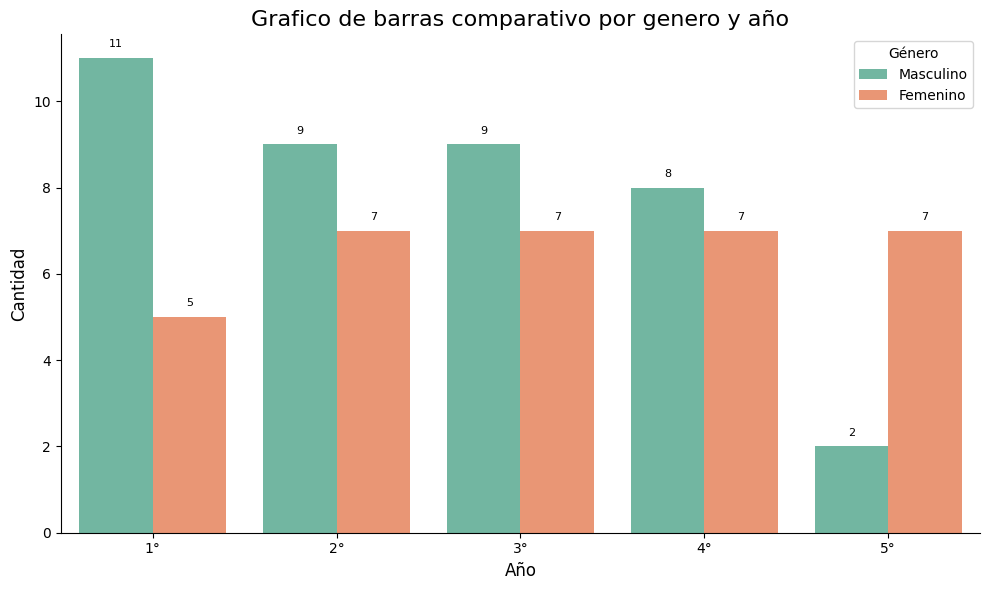
\includegraphics[width=0.80\textwidth]{images/GeneroPorAño.png}
    \end{center}
    \label{fig:GeneroPorAño}
    \caption{Comparación de la distribución de género por año de estudio}
\end{figure}

\textbf{Interpretación}
El análisis de género por año de estudio revela patrones interesantes:
\begin{itemize}
    \item En primer año se observa una distribución equilibrada entre géneros
    \item Existe una predominancia femenina en el segundo y tercer año
    \item En los años superiores (cuarto y quinto) hay una mayor presencia masculina
    \item La distribución general muestra una ligera mayoría masculina en la población estudiantil total
\end{itemize}

\subsection{Analisis brecha digital}

\subsubsection{Acceso}

\begin{figure}[H]
    \begin{center}
        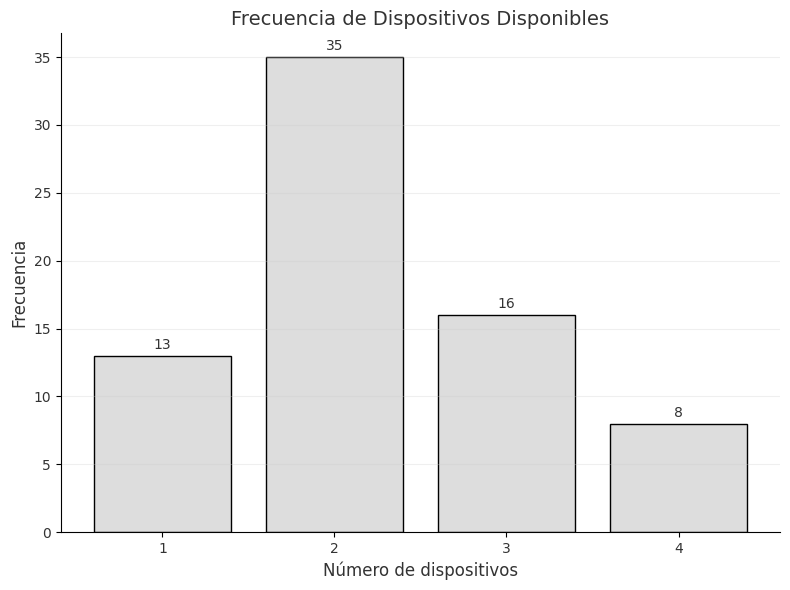
\includegraphics[width=0.80\textwidth]{images/DispositivosDisponibles.png}
    \end{center}
    \label{fig:DispositivosDisponibles}
    \caption{Frecuencia de dispositivos disponibles}
\end{figure}

\textbf{Interpretación}
\subsubsection{Acceso a dispositivos}
El análisis de la cantidad de disponibles muestra:
\begin{itemize}
    \item La mayoría de los estudiantes tienen 2 dispositivos disponibles.
    \item A medida que el número de dispositivos aumenta (más de 3), la frecuencia disminuye.
    \item Esto indica que la disponibilidad de más dispositivos es menos común.
\end{itemize}

\begin{figure}[H]
    \begin{center}
        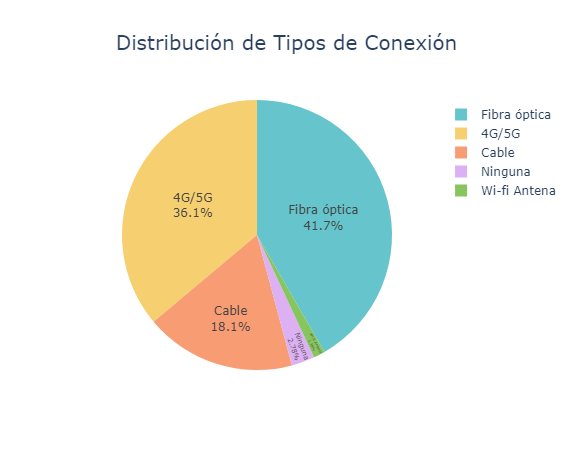
\includegraphics[width=0.80\textwidth]{images/DistribucionConexion.png}
    \end{center}
    \label{fig:DistribucionConexion}
    \caption{Tipos de conexión a intenet}
\end{figure}

\textbf{Interpretación}
En cuanto a los tipos de conexión:
\begin{itemize}
    \item El plan móvil es el método predominante (aproximadamente 45\%)
    \item La conexión por WiFi doméstico representa cerca del 35\%
    \item Los planes compartidos constituyen alrededor del 15\%
    \item Existe un pequeño porcentaje que depende de conexiones públicas o gratuitas
\end{itemize}

\begin{figure}[H]
    \begin{center}
        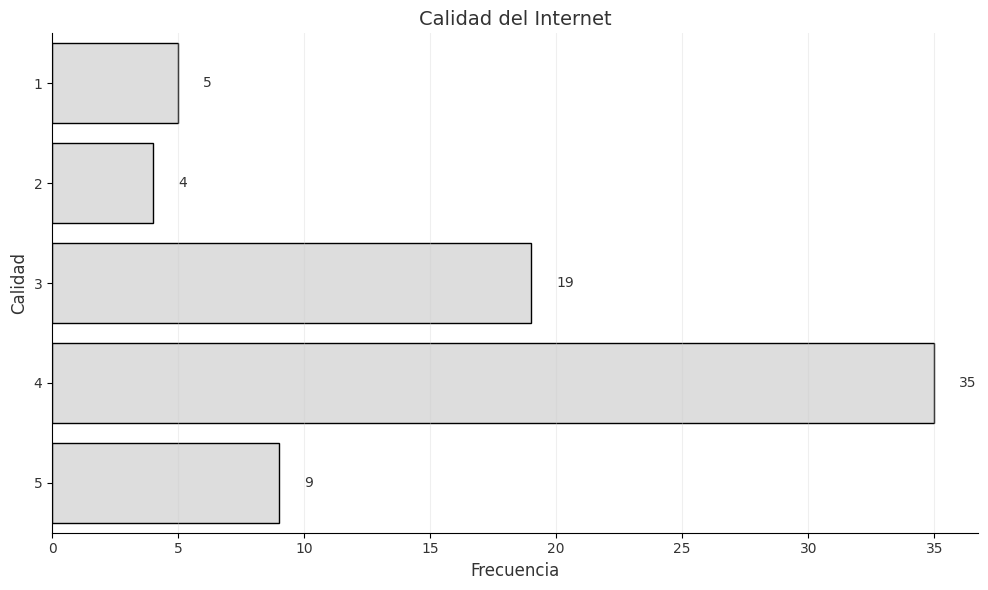
\includegraphics[width=0.80\textwidth]{images/FrecuenciaCalidadInternet.png}
    \end{center}
    \label{fig:FrecuenciaCalidadInternet}
    \caption{Grafico de barras de la calida de internet}
\end{figure}

\textbf{Interpretación}
La calidad del internet muestra una distribución preocupante:
\begin{itemize}
    \item Solo el 20\% reporta una conexión de alta calidad
    \item La mayoría (aproximadamente 45\%) indica una calidad media
    \item Un significativo 35\% experimenta conexión de baja calidad
\end{itemize}

\subsubsection{Uso}

\begin{table}[H]
    \centering

    \begin{tabular}{llccccccc}
        \toprule
        \textbf{Index} & \textbf{Intervalos} & \textbf{mi} & \textbf{fi} & \textbf{Fi} & \textbf{hi} & \textbf{Hi} & \textbf{pi (\%)} & \textbf{Pi (\%)} \\
        \midrule
        1 & [ 30.0 - 77.0 )  & 53.5  & 13 & 13 & 0.181 & 0.181 & 18.1 & 18.1 \\
        2 & [ 77.0 - 124.0 ) & 100.5 & 14 & 27 & 0.194 & 0.375 & 19.4 & 37.5 \\
        3 & [ 124.0 - 171.0 ) & 147.5 & 11 & 38 & 0.153 & 0.528 & 15.3 & 52.8 \\
        4 & [ 171.0 - 218.0 ) & 194.5 & 14 & 52 & 0.194 & 0.722 & 19.4 & 72.2 \\
        5 & [ 218.0 - 265.0 ) & 241.5 & 9  & 61 & 0.125 & 0.847 & 12.5 & 84.7 \\
        6 & [ 265.0 - 312.0 ) & 288.5 & 2  & 63 & 0.028 & 0.875 & 2.8  & 87.5 \\
        7 & [ 312.0 - 359.0 ) & 335.5 & 3  & 66 & 0.042 & 0.917 & 4.2  & 91.7 \\
        8 & [ 359.0 - 406.0 ] & 382.5 & 6  & 72 & 0.083 & 1.000	 & 8.3  & 100.0 \\
        \bottomrule
    \end{tabular}
    \vspace{0.1cm}
    \caption{Tabla de distribución de frecuencia (\textbf{minutos} al día) en el uso de TIC con fines educativos}
    \label{tab:frecuenciaUso}
\end{table}

\textbf{Pincipales estadisticos}

\begin{itemize}
    \item Media: 171.8056
    \item Moda: 200
    \item Mediana: 170
    \item Varianza: 10245.9898
    \item Desviación estandar: 101.2225
\end{itemize}

\begin{figure}[H]
    \begin{center}
        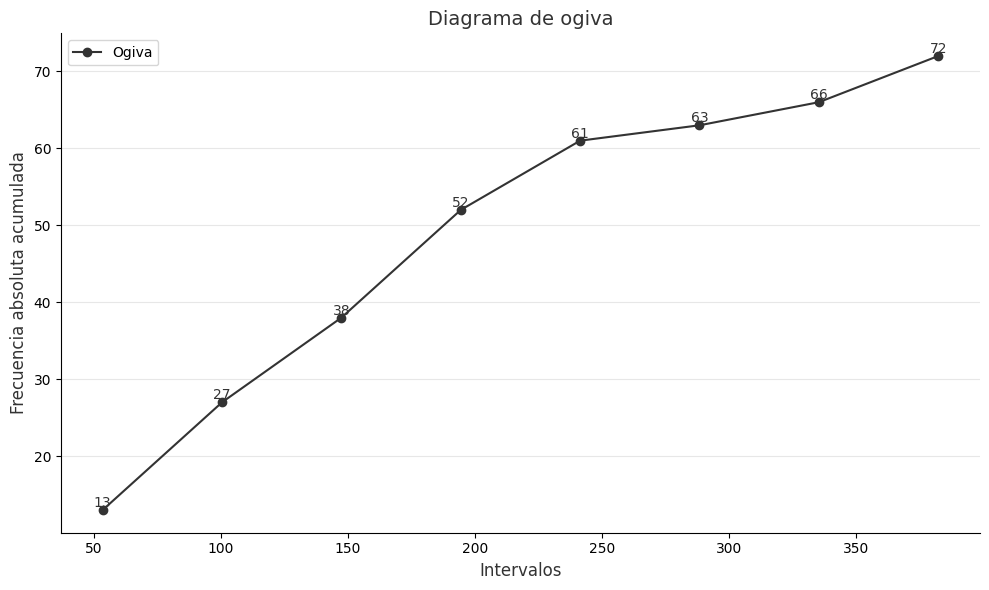
\includegraphics[width=0.80\textwidth]{images/DiagramOgiva.png}
    \end{center}
    \label{fig:DiagramOgiva}
    \caption{Ogiva de frecuencia absoluta acumulada}
\end{figure}

\textbf{Interpretación}
El análisis del tiempo de uso diario revela:
\begin{itemize}
    \item Una media de 171.81 minutos (aproximadamente 2.86 horas)
    \item Una desviación estándar alta de 100.52 minutos, indicando gran variabilidad
    \item El 72.2\% de los estudiantes utiliza dispositivos digitales menos de 218 minutos diarios
    \item Solo el 8.3\% reporta un uso superior a 359 minutos
\end{itemize}

\begin{figure}[H]
    \begin{center}
        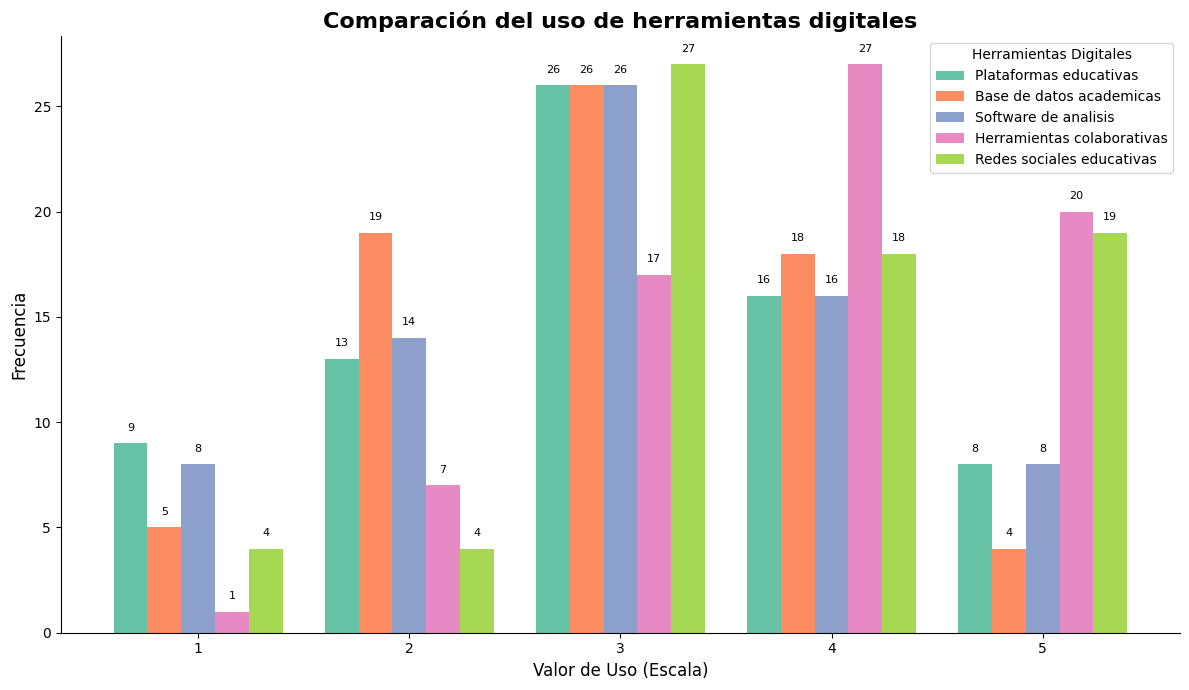
\includegraphics[width=0.80\textwidth]{images/PropositoUso.png}
    \end{center}
    \label{fig:PropositoUso}
    \caption{Comparación de proposito de uso}
\end{figure}

Los principales propósitos de uso se distribuyen de la siguiente manera:
\begin{itemize}
    \item Actividades académicas: predominante con aproximadamente 45\%
    \item Comunicación: segundo uso más común con 25\%
    \item Entretenimiento: representa aproximadamente 20\%
    \item Otros usos: constituyen el 10\% restante
\end{itemize}

\subsubsection{Habilidades Digitales}

\begin{figure}[H]
    \begin{center}
        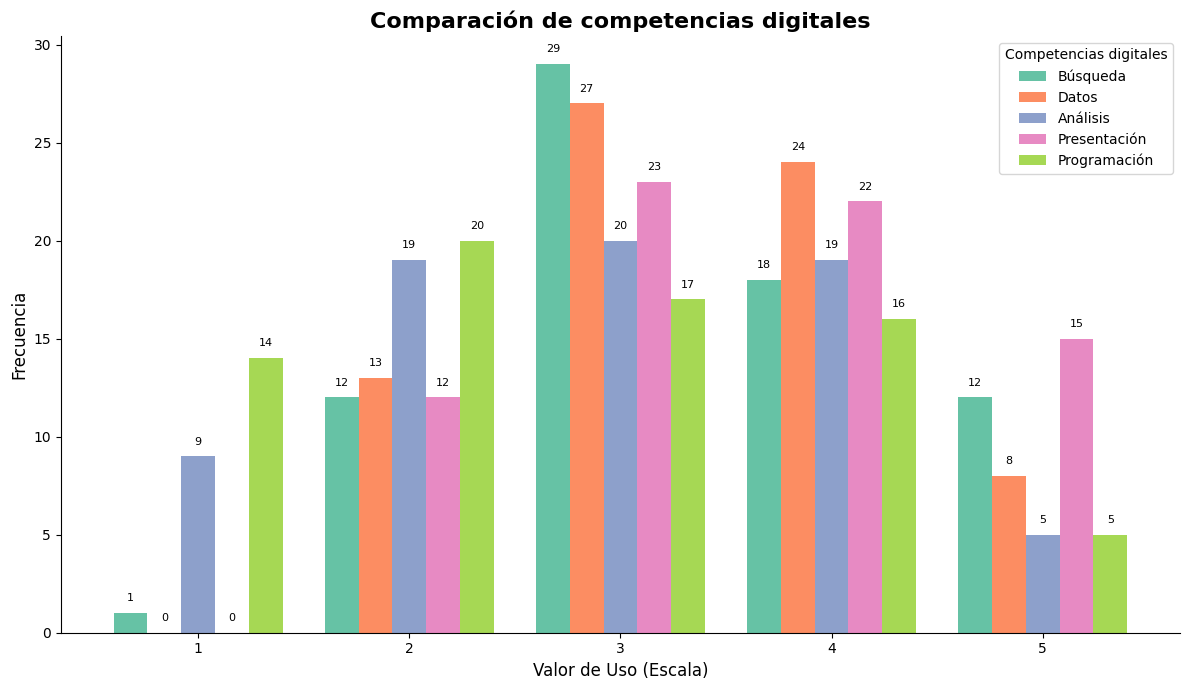
\includegraphics[width=0.80\textwidth]{images/CompetenciasDigitales.png}
    \end{center}
    \label{fig:CompetenciasDigitales}
    \caption{Comparación de habilidades digitales (escala)}
\end{figure}

\textbf{Interpretación}

La evaluación de competencias digitales muestra una distribución heterogénea:
\begin{itemize}
    \item Habilidades básicas (navegación web, correo electrónico): nivel alto (>75\%)
    \item Habilidades intermedias (ofimática, redes sociales): nivel medio-alto (60-75\%)
    \item Habilidades avanzadas (programación, análisis de datos): nivel bajo (<40\%)
\end{itemize}

Esta distribución sugiere una brecha significativa en habilidades digitales avanzadas, especialmente en aquellas relevantes para el campo de la economía.


\subsection{Implicaciones}
Los resultados sugieren una brecha digital multidimensional:
\begin{enumerate}
    \item \textbf{Acceso}: Aunque existe alta penetración de dispositivos móviles, hay limitaciones en el acceso a equipos más apropiados para trabajo académico.
    \item \textbf{Conectividad}: La dependencia de planes móviles y la calidad variable de internet pueden afectar el desempeño académico.
    \item \textbf{Habilidades}: Existe una clara necesidad de fortalecimiento en competencias digitales avanzadas.
\end{enumerate}

\section{Conclusiones y recomendaciones}

\subsection{Síntesis de hallazgos principales}

Los resultados de esta investigación sobre la brecha digital en los estudiantes de la Facultad de Economía de la Unheval revelan varios hallazgos significativos:

\begin{enumerate}
    \item \textbf{Perfil demográfico}
    \begin{itemize}
        \item La población estudiantil es predominantemente joven (edad media 20.73 años)
        \item Existe una distribución de género variable según el año de estudio
        \item La mayor concentración de estudiantes se encuentra entre 21-22 años (25\%)
    \end{itemize}

    \item \textbf{Acceso a tecnología}
    \begin{itemize}
        \item La mayoría de los estudiantes tienen 2 dispositivos disponibles.
        \item Predominio de conexiones móviles sobre conexiones fijas domiciliarias
    \end{itemize}

    \item \textbf{Patrones de uso}
    \begin{itemize}
        \item Tiempo promedio de uso diario: 2.86 horas
        \item Predominio de uso académico (45\% del tiempo)
        \item Alta variabilidad en tiempos de uso (DE = 100.52 minutos)
    \end{itemize}
\end{enumerate}

\subsection{Conclusiones}

\subsubsection{Sobre el acceso digital}

\begin{enumerate}
    \item La brecha de acceso se manifiesta principalmente en la calidad de los dispositivos y la conectividad, más que en la posesión de dispositivos básicos.
    
    \item La dependencia de conexiones móviles sugiere una vulnerabilidad en la continuidad del acceso digital, potencialmente afectando el desempeño académico.
    
    \item La calidad heterogénea de la conexión a internet (solo 20\% reporta alta calidad) representa una barrera significativa para el aprovechamiento de recursos educativos digitales.
\end{enumerate}

\subsubsection{Sobre las competencias digitales}

\begin{enumerate}
    \item Existe una brecha significativa entre las habilidades básicas y avanzadas, siendo estas últimas críticas para el campo de la economía.
    
    \item La concentración en habilidades básicas sugiere una formación digital insuficiente para las demandas del mercado laboral actual.
    
    \item Las competencias en análisis de datos y programación son particularmente deficientes, lo cual es preocupante para estudiantes de economía.
\end{enumerate}

\subsection{Recomendaciones}

\subsubsection{Para la institución}

\begin{enumerate}
    \item \textbf{Infraestructura tecnológica}
    \begin{itemize}
        \item Implementar laboratorios de cómputo con software especializado para economía
        \item Mejorar la red WiFi del campus en términos de cobertura y velocidad
        \item Establecer convenios con proveedores de servicios de internet para planes estudiantiles
    \end{itemize}

    \item \textbf{Desarrollo de competencias}
    \begin{itemize}
        \item Incorporar cursos obligatorios de análisis de datos y programación
        \item Implementar talleres extracurriculares de habilidades digitales avanzadas
        \item Desarrollar un programa de certificación en competencias digitales
    \end{itemize}

    \item \textbf{Apoyo estudiantil}
    \begin{itemize}
        \item Crear un programa de préstamo de laptops para estudiantes de bajos recursos
        \item Establecer un sistema de tutoría entre pares para habilidades digitales
        \item Implementar un centro de recursos digitales con asesoría técnica
    \end{itemize}
\end{enumerate}

\subsubsection{Para los estudiantes}

\begin{enumerate}
    \item \textbf{Desarrollo personal}
    \begin{itemize}
        \item Aprovechar recursos gratuitos en línea para el desarrollo de habilidades digitales
        \item Participar activamente en talleres y programas de capacitación ofrecidos
        \item Formar grupos de estudio para el aprendizaje colaborativo de herramientas digitales
    \end{itemize}

    \item \textbf{Gestión de recursos}
    \begin{itemize}
        \item Priorizar la inversión en dispositivos apropiados para el trabajo académico
        \item Optimizar el uso del tiempo en línea para actividades académicas
        \item Explorar opciones de conectividad más estables y económicas
    \end{itemize}
\end{enumerate}

\subsubsection{Para futuras investigaciones}

\begin{enumerate}
    \item Realizar estudios longitudinales para evaluar la evolución de la brecha digital
    \item Investigar el impacto de las intervenciones institucionales en las competencias digitales
    \item Desarrollar métricas más precisas para evaluar habilidades digitales específicas del campo económico
    \item Analizar la correlación entre competencias digitales y rendimiento académico
\end{enumerate}

\subsection{Consideraciones finales}

La reducción de la brecha digital requiere un enfoque integral que aborde simultáneamente el acceso a tecnología, el desarrollo de competencias y el apoyo institucional. El éxito de estas intervenciones dependerá de la colaboración activa entre la institución, los docentes y los estudiantes, así como del compromiso con la transformación digital de la educación superior en economía.

\newpage
\printbibliography

\newpage
\appendix
\addcontentsline{toc}{section}{Anexos}

\subsection*{Anexo A: Encuesta aplicada}

\subsubsection*{I. Datos demográficos y académicos}
\begin{enumerate}[label=\arabic*.]
    \item Edad: \_\_\_\_
    \item Género: \hspace{1em} $\square$ Masculino \hspace{1em} $\square$ Femenino
    \item Año de estudio: \\ $\square$ 1° \hspace{1em}  $\square$ 2° 
    \hspace{1em}  $\square$ 3° \hspace{1em} 
         $\square$ 4° \hspace{1em} 
         $\square$ 5°

\end{enumerate}

\subsubsection*{II. Acceso a dispositivos y conectividad}
\begin{enumerate}[resume, label=\arabic*.]
    \item ¿Qué dispositivos posees? (Marca todos los que apliquen)\\
    $\square$ Smartphone \hspace{1em} $\square$ Laptop \hspace{1em} $\square$ Tablet \hspace{1em} $\square$ Computadora de escritorio \hspace{1em} $\square$ Otro: \_\_\_\_\_
    \item ¿Qué tipo de conexión a internet tienes en casa?\\
    $\square$ Fibra óptica \hspace{1em} $\square$ ADSL \hspace{1em} $\square$ Cable \hspace{1em} $\square$ 4G/5G \hspace{1em} $\square$ Ninguna \hspace{1em} $\square$ Otro: \_\_\_\_\_
    \item En una escala del 1 al 5, ¿cómo calificarías la calidad de tu conexión a internet?\\
    Muy mala \hspace{1em} 1 $\square$ \hspace{1em} 2 $\square$ \hspace{1em} 3 $\square$ \hspace{1em} 4 $\square$ \hspace{1em} 5 $\square$ Excelente
\end{enumerate}

\subsubsection*{III. Frecuencia y tipo de uso de TIC en actividades académicas}
\begin{enumerate}[resume, label=\arabic*.]
    \item ¿Con qué frecuencia utilizas los siguientes recursos digitales para tus estudios?\\
    (1: Nunca, 2: Rara vez, 3: A veces, 4: Frecuentemente, 5: Siempre)
    \begin{itemize}
        \item Plataforma educativa de la universidad (ej. Moodle)\\
        \hspace{1em} 1 $\square$ \hspace{1em} 2 $\square$ \hspace{1em} 3 $\square$ \hspace{1em} 4 $\square$ \hspace{1em} 5 $\square$
        \item Bases de datos académicas (ej. JSTOR, EconLit)\\
        \hspace{1em} 1 $\square$ \hspace{1em} 2 $\square$ \hspace{1em} 3 $\square$ \hspace{1em} 4 $\square$ \hspace{1em} 5 $\square$
        \item Software de análisis estadístico (ej. STATA, R)\\
        \hspace{1em} 1 $\square$ \hspace{1em} 2 $\square$ \hspace{1em} 3 $\square$ \hspace{1em} 4 $\square$ \hspace{1em} 5 $\square$
        \item Herramientas de colaboración en línea (ej. Google Docs)\\
        \hspace{1em} 1 $\square$ \hspace{1em} 2 $\square$ \hspace{1em} 3 $\square$ \hspace{1em} 4 $\square$ \hspace{1em} 5 $\square$
        \item Redes sociales con fines académicos\\
        \hspace{1em} 1 $\square$ \hspace{1em} 2 $\square$ \hspace{1em} 3 $\square$ \hspace{1em} 4 $\square$ \hspace{1em} 5 $\square$
    \end{itemize}
    \item En promedio, ¿cuántos minutos al día dedicas al uso de TIC para actividades académicas?\\
    \_\_\_\_\_\_\_\_\_
\end{enumerate}

\subsubsection*{IV. Competencias digitales autopercibidas}
\begin{enumerate}[resume, label=\arabic*.]
    \item Evalúa tu nivel de habilidad en las siguientes competencias digitales:\\
    (1: Nulo, 2: Básico, 3: Intermedio, 4: Avanzado, 5: Experto)
    \begin{itemize}
        \item Búsqueda y evaluación de información en línea\\
        \hspace{1em} 1 $\square$ \hspace{1em} 2 $\square$ \hspace{1em} 3 $\square$ \hspace{1em} 4 $\square$ \hspace{1em} 5 $\square$
        \item Uso de software de hojas de cálculo (ej. Excel)\\
        \hspace{1em} 1 $\square$ \hspace{1em} 2 $\square$ \hspace{1em} 3 $\square$ \hspace{1em} 4 $\square$ \hspace{1em} 5 $\square$
        \item Análisis de datos con software especializado\\
        \hspace{1em} 1 $\square$ \hspace{1em} 2 $\square$ \hspace{1em} 3 $\square$ \hspace{1em} 4 $\square$ \hspace{1em} 5 $\square$
        \item Creación de presentaciones multimedia\\
        \hspace{1em} 1 $\square$ \hspace{1em} 2 $\square$ \hspace{1em} 3 $\square$ \hspace{1em} 4 $\square$ \hspace{1em} 5 $\square$
        \item Programación (ej. Python, R)\\
        \hspace{1em} 1 $\square$ \hspace{1em} 2 $\square$ \hspace{1em} 3 $\square$ \hspace{1em} 4 $\square$ \hspace{1em} 5 $\square$
    \end{itemize}
\end{enumerate}

\subsection*{Anexo B: Matriz de operacionalización de variables}

\begin{landscape}
    \begin{figure}[H]
        \begin{center}
            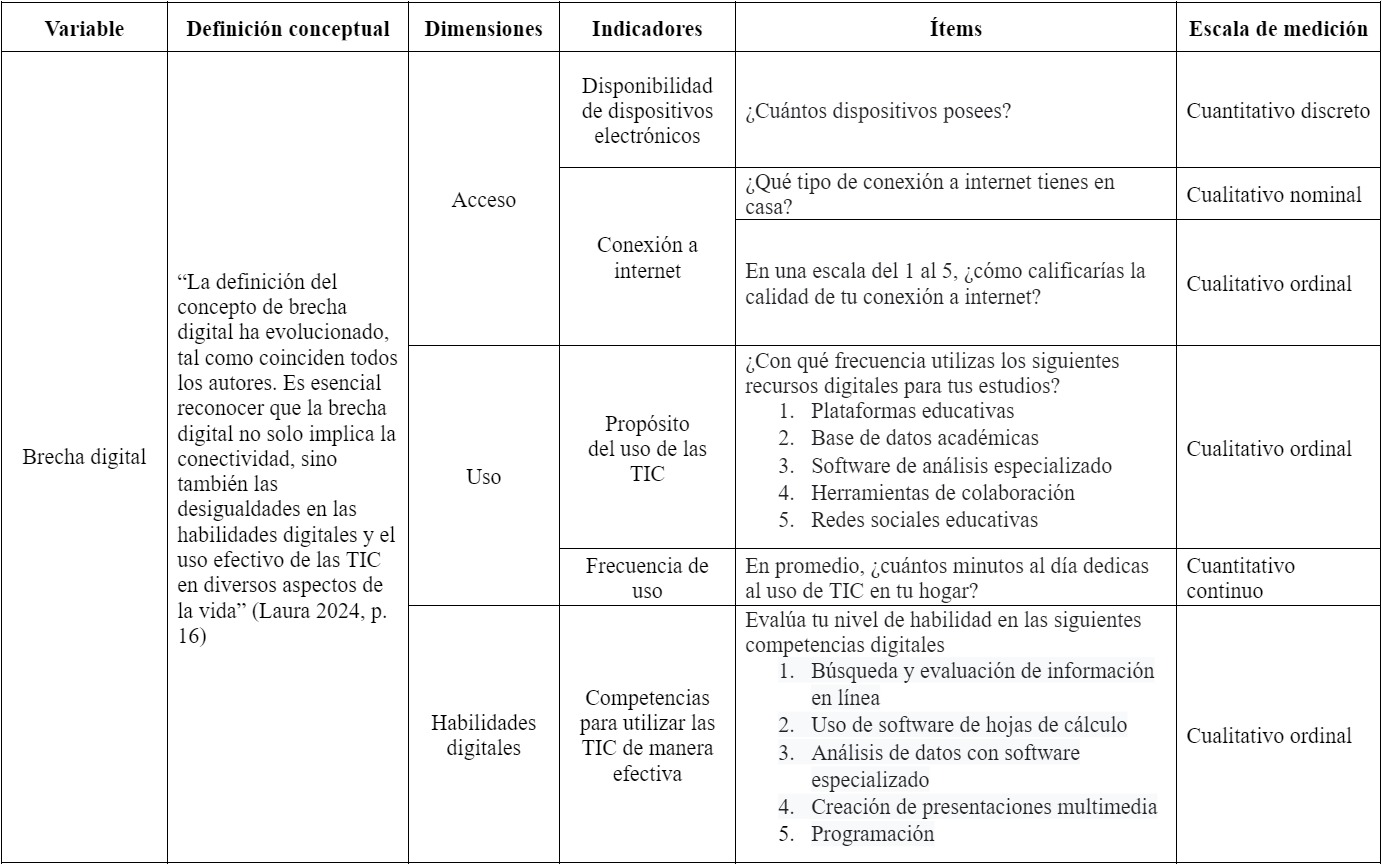
\includegraphics[width=1.4\textwidth]{images/MatrizOperacionalizacion.jpg}
        \end{center}
        \label{fig:MatrizOperacionalizacion}
        \caption{Matriz de operacionalización de variables}
    \end{figure}
\end{landscape}

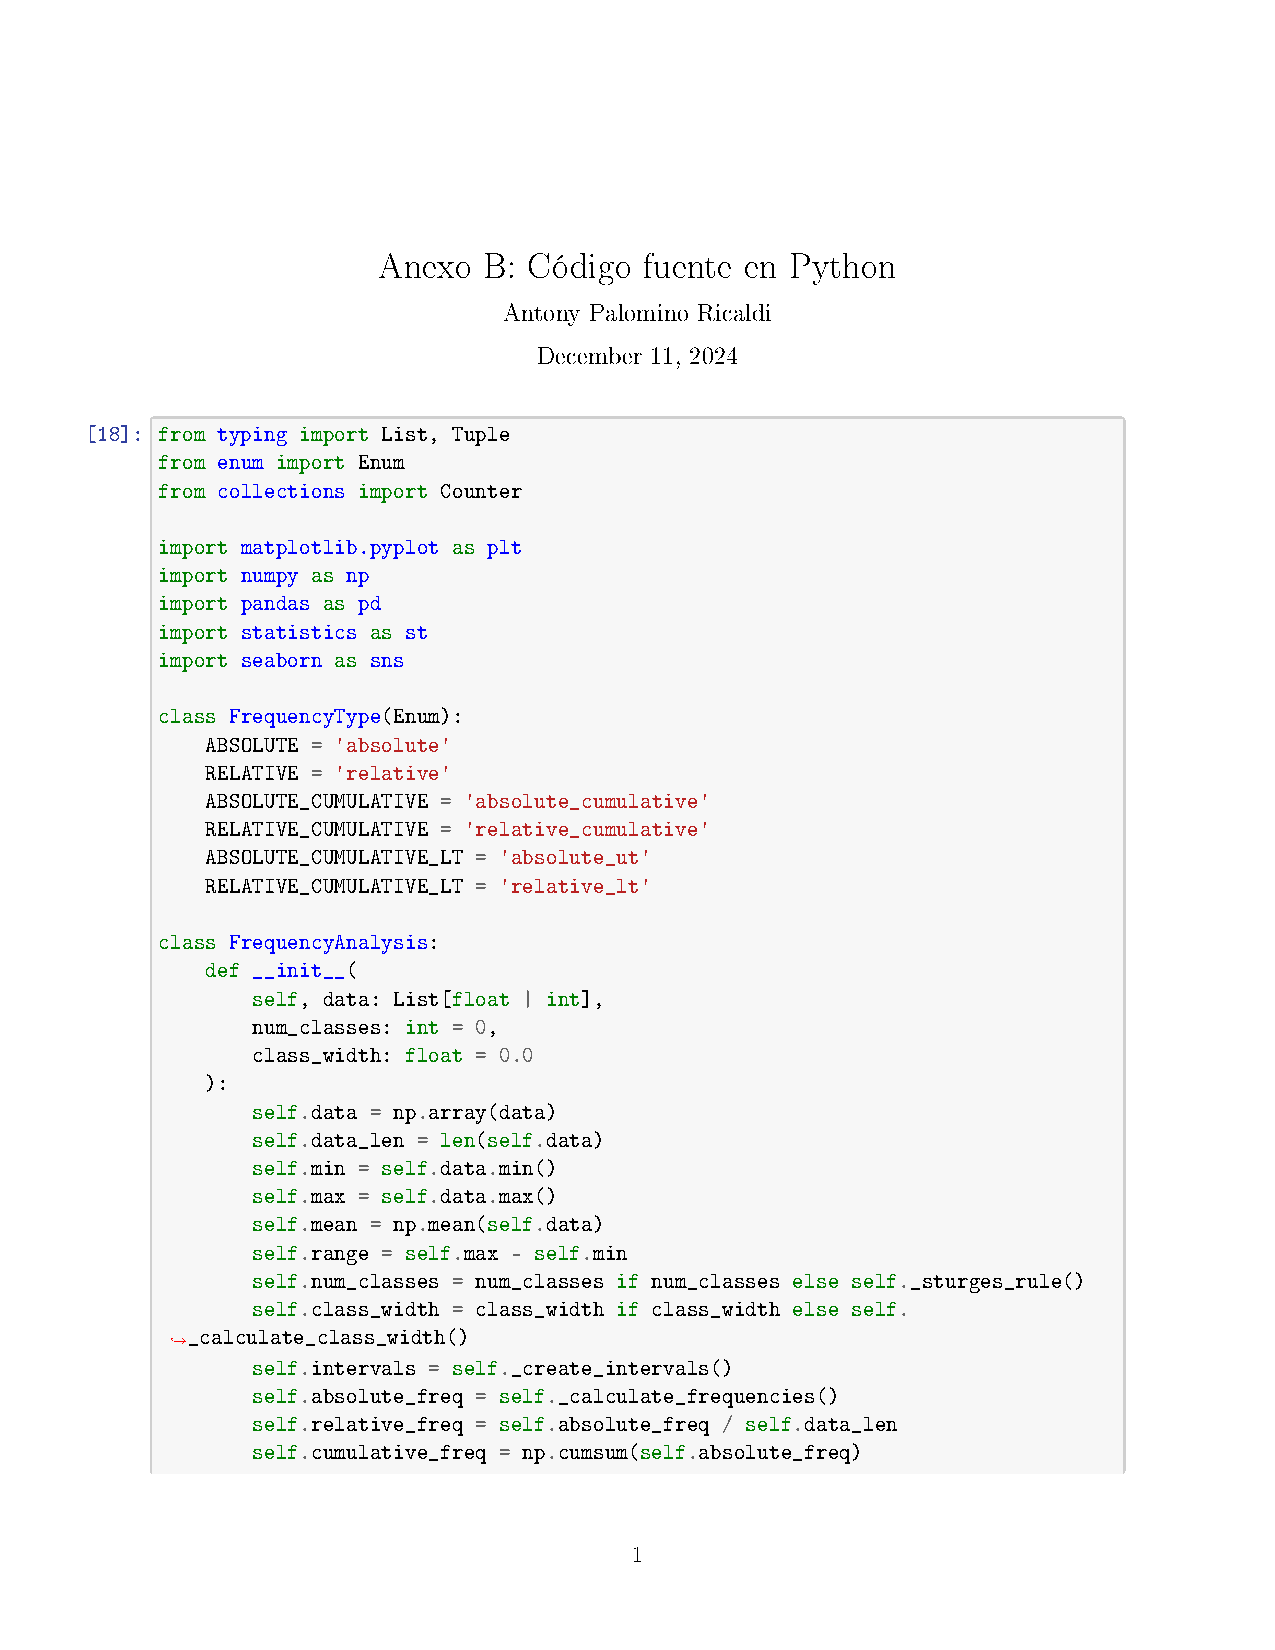
\includepdf[pages=-]{codigo.pdf}
\end{document}